\documentclass[conference,letterpaper]{IEEEtran}
\usepackage{cite}
\usepackage{amsmath}
\usepackage{graphicx}
\usepackage{tikz}
\usetikzlibrary{arrows.meta,positioning}
\usepackage{url}
\usepackage{booktabs}

\begin{document}

\title{Measuring Cross-Dataset Fake-News Detection under Leave-One-Dataset-Out Evaluation}

\author{\IEEEauthorblockN{Lekhraj and Shreyash Shrikant Yadav}
\IEEEauthorblockA{M.Tech, Artificial Intelligence and Machine Learning}}

\maketitle

\begin{abstract}
A text classifier can score well on the dataset used for training and worse on another dataset when writing style, topic, and the meaning of the binary label change together. This paper measures that gap on three processed datasets: 6,000 refined ISOT articles, 12,759 LIAR-PLUS claims, and 478 Fake-versus-Satire texts. TF-IDF with logistic regression, fit by scikit-learn, and DistilBERT, trained by Hugging Face Transformers, use seed 42. Each model is tested in-domain and leave-one-dataset-out on the same target test split. Macro-F1 is the primary metric. DistilBERT in-domain macro-F1 is 0.9889, 0.6238, and 0.7312. Leave-one-dataset-out macro-F1 is 0.5867, 0.3778, and 0.3917. On all three leave-one-dataset-out targets, TF-IDF with logistic regression is higher in this single-seed run. An uncertainty rule at thresholds 0.3, 0.4, and 0.5, applied by the analysis script to saved DistilBERT probabilities, does not restore the scores. LoRA adaptation with 16 target training labels, applied with PEFT to the leave-one-dataset-out checkpoints, likewise does not restore them. A separate nine-source DistilBERT run, which does not overwrite the locked runs, records macro-F1 of 0.6677, 0.3544, and 0.7103 on the same three tests. Only one seed was used.
\end{abstract}

\begin{IEEEkeywords}
fake news, leave-one-dataset-out, DistilBERT, TF-IDF, LoRA, selective prediction
\end{IEEEkeywords}

\section{Introduction}
A detector of misleading text is often judged on a single collection. That test answers a narrow question: after training on one distribution, how well does the model label a held-out part of the same collection? A second collection can differ in topic, in article length, and in what the positive class means. A claim marked half-true is not the same object as a fabricated news article, and a satire piece is not a real report. A score that looks strong inside one collection can therefore fall when the test collection changes.

This study measures that fall. It does not claim a new detector that removes it. The measured objects are two fixed classifiers, one shared test rule, one post-hoc abstention rule, and one small adapter. All reported scores come from saved prediction and metric files. No score in this paper is estimated from a run that was not saved.

The study makes four contributions.
\begin{enumerate}
\item It compares TF-IDF plus logistic regression with DistilBERT on three datasets under in-domain testing and leave-one-dataset-out (LODO) testing, using the same target test split for both tests.
\item It applies a fixed uncertainty score, $\mathrm{compatibility}=1-H(p)/\ln 2$, to saved LODO probabilities at the preset thresholds 0.3, 0.4, and 0.5.
\item It compares guided and random LoRA adaptation that each use 16 labels drawn only from the target training split.
\item It records a separate nine-source DistilBERT LODO result on the same three target tests without changing the first ten neural runs.
\end{enumerate}

\section{Related Work}
Dell'Oglio, Bondielli, Marcelloni, and Passaro compare popular fake-news detectors across multiple datasets and report that a strong in-domain score is a weak guide to a cross-dataset score~\cite{delloglio2026}. Their comparison is the starting point for the protocol in this paper. This study is not a reproduction of that paper. It uses DistilBERT rather than the full model list, a balanced 6,000-row ISOT subsample rather than the full refined file, and one random seed. Their published scores are not copied into our tables.

DistilBERT is the distilled encoder used for the neural runs~\cite{sanh2019}. Low-rank adaptation (LoRA) is the adapter used for the four small updates~\cite{hu2022}. The linear baseline is a TF-IDF vectorizer followed by $\ell_2$-regularized logistic regression, as implemented in scikit-learn~\cite{pedregosa2011}. Neural training and tokenization use the Transformers library~\cite{wolf2020}. These tools are credited only for the stages they actually execute. scikit-learn fits the TF-IDF baseline and supplies the accuracy and macro-F1 functions. Transformers trains DistilBERT and writes its predictions. PEFT attaches the LoRA adapters. The analysis script reads saved predictions and computes coverage and risk; it does not train a model.

The text collections are an existing refined ISOT variant~\cite{isotuvic,phoenyx83}, the LIAR-PLUS claim files~\cite{liarplus}, and a local Fake-versus-Satire archive restricted to its final fake and final satire directories. Seven further processed collections are used only in the extra nine-source run: Celebrity, Cidii, Fakes, Horne, Infodemic, NDF, and Politifact.

\section{Proposed Methodology and System Architecture}
Figure~\ref{fig:pipeline} shows the path from a raw file to a saved score. Each box names the stage and the program that performs it.

\begin{figure}[t]
\centering
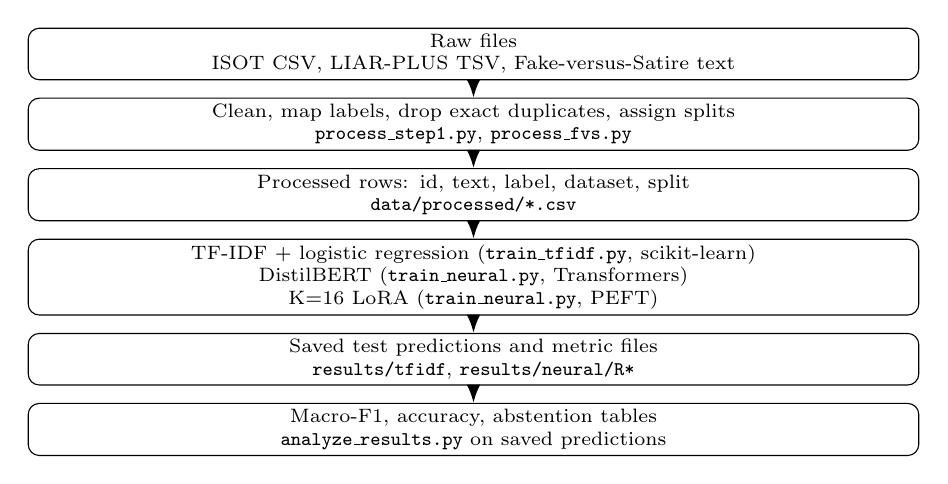
\begin{tikzpicture}[
  node distance=2.2mm,
  box/.style={draw, rounded corners, align=center, font=\scriptsize,
              inner sep=2.2pt, text width=0.92\columnwidth},
  arr/.style={-{Latex}, thick}
]
\node[box] (raw) {Raw files\\ ISOT CSV, LIAR-PLUS TSV, Fake-versus-Satire text};
\node[box, below=of raw] (prep) {Clean, map labels, drop exact duplicates, assign splits\\ \texttt{process\_step1.py}, \texttt{process\_fvs.py}};
\node[box, below=of prep] (csv) {Processed rows: id, text, label, dataset, split\\ \texttt{data/processed/*.csv}};
\node[box, below=of csv] (models) {TF-IDF + logistic regression (\texttt{train\_tfidf.py}, scikit-learn)\\ DistilBERT (\texttt{train\_neural.py}, Transformers)\\ K=16 LoRA (\texttt{train\_neural.py}, PEFT)};
\node[box, below=of models] (pred) {Saved test predictions and metric files\\ \texttt{results/tfidf}, \texttt{results/neural/R*}};
\node[box, below=of pred] (score) {Macro-F1, accuracy, abstention tables\\ \texttt{analyze\_results.py} on saved predictions};
\draw[arr] (raw) -- (prep);
\draw[arr] (prep) -- (csv);
\draw[arr] (csv) -- (models);
\draw[arr] (models) -- (pred);
\draw[arr] (pred) -- (score);
\end{tikzpicture}
\caption{Pipeline from raw files to saved scores. Preparation scripts do not compute macro-F1. The analysis script does not train.}
\label{fig:pipeline}
\end{figure}

\subsection{Data preparation}
\texttt{process\_step1.py} reads the ISOT and LIAR-PLUS files with the Python standard library. For ISOT it keeps the article body, strips a leading Reuters dateline and the phrase ``21st Century Wire says,'' and maps a real article to 0 and a fake article to 1. For LIAR-PLUS it keeps the claim text only. The labels pants-fire, false, and barely-true map to 1. The labels half-true, mostly-true, and true map to 0. Exact normalized duplicates are removed. ISOT is then subsampled with seed 42 to 3,000 rows per class and split 2,100/450/450. LIAR-PLUS keeps its official train, validation, and test assignment after cleaning.

\texttt{process\_fvs.py} reads only \texttt{finalFake} and \texttt{finalSatire}. Fake maps to 1 and satire maps to 0. URL strings are removed before classification so a domain name is not a feature. Rows with fewer than 20 words are dropped. The remaining rows are split with seed 42 into about 70\% train, 15\% validation, and 15\% test. Neither preparation script trains a classifier or writes a macro-F1 score.

\subsection{Classifiers}
The baseline script builds a scikit-learn pipeline: word unigrams and bigrams, at most 50,000 features, minimum document frequency 2, sublinear term frequency, and logistic regression with $C=1$, the liblinear solver, and a maximum of 1,000 iterations. The vectorizer is fit on training text only. Seed 42 is fixed. In-domain training uses the target training split. LODO training uses the training splits of the other datasets and never the target training, validation, or test rows. The test split is the target test split in both protocols.

DistilBERT-base-uncased is fine-tuned for two epochs at learning rate $2\times10^{-5}$, batch size 4, maximum length 128, seed 42, and fp16, as set in \texttt{train\_neural.py}. Runs R1--R3 are in-domain. Runs R4--R6 are LODO. The source list is stored in each \texttt{metrics.json}. R4 trains on LIAR-PLUS and Fake versus Satire and tests on ISOT. R5 trains on ISOT and Fake versus Satire and tests on LIAR-PLUS. R6 trains on ISOT and LIAR-PLUS and tests on Fake versus Satire.

\subsection{Abstention and LoRA}
After training, \texttt{analyze\_results.py} reads the saved DistilBERT probabilities. For a two-class probability vector $p$ it computes
\begin{equation}
\mathrm{compatibility}=1-\frac{H(p)}{\ln 2},
\quad H(p)=-\sum_i p_i\ln p_i.
\end{equation}
The script answers when the score is at least $t$ and abstains otherwise, for every $t\in\{0.3,0.4,0.5\}$. These thresholds were fixed before looking for a best test score. Coverage is the fraction of target test rows that receive an answer. Risk is the fraction of answered rows that are wrong. The script also reports macro-F1 on the answered rows. This score measures peaked probabilities. It does not measure whether two datasets use the same meaning of ``real.''

Runs R7--R10 start from a finished LODO checkpoint, not from a fresh DistilBERT. R7 and R9 load R5. R8 and R10 load R6. Each adapter is trained on 16 rows from the target training split only. Guided selection keeps the 16 training rows with the highest predictive entropy under the source model. Random selection draws 16 rows with seed 42. PEFT uses rank 8, alpha 16, dropout 0.1, and target modules \texttt{q\_lin} and \texttt{v\_lin}. The classification head remains trainable. Target test labels are not used to choose the 16 rows.

\subsection{Separate nine-source run}
\texttt{train\_lodo10.py} trains additional DistilBERT models on the processed collections that are present on disk. It is written so that it does not overwrite R1--R10. For a held-out target, the training pool is the training splits of the other nine collections. The test set remains that target's original test split. The three numbers used below are the saved macro-F1 values for ISOT, LIAR-PLUS, and Fake versus Satire.

\section{Experimental Setup}
\subsection{Datasets}
Table~\ref{tab:data} gives the processed sizes. ISOT test rows are balanced, 450 per class. LIAR-PLUS test rows contain 714 of class 0 and 553 of class 1. Fake versus Satire test rows contain 31 satire texts and 42 fake texts. The processed columns are id, text, label, dataset, and split. There is no user identifier, so the study has no user-wise split and does not report a second table by user.

The ISOT input is the Phoenyx83 refined 2022 variant, with 17,058 real rows and 17,050 fake rows before cleaning, not the untouched full release. After cleaning, 34,099 unique rows remain and the seed-42 sample keeps 6,000. LIAR-PLUS starts from 12,793 parsed records and keeps 12,759. Fake versus Satire starts from 486 final text files and keeps 478. Exact normalized duplicates were removed. Near-duplicate sentences were not checked.

\begin{table}[t]
\caption{Processed dataset sizes and label meanings.}
\label{tab:data}
\centering
\scriptsize
\begin{tabular}{lrrrl}
\hline
Dataset & Train & Val & Test & Class 0 \\
\hline
ISOT & 4200 & 900 & 900 & Real article \\
LIAR-PLUS & 10208 & 1284 & 1267 & Half-true group \\
Fake vs.\ Satire & 334 & 71 & 73 & Satire \\
\hline
\end{tabular}
\end{table}

Class 1 is Fake for ISOT and Fake versus Satire. For LIAR-PLUS, class 1 is pants-fire, false, or barely-true. Class 0 on LIAR-PLUS includes half-true claims, so it is not a guarantee of factual truth. Satire is not a real news article.

\subsection{Test rule}
Macro-F1 is primary. Accuracy is reported beside it. In-domain and LODO comparisons use the same target test rows. LODO validation, where used for checkpoint selection, comes from the source datasets, not from the target. Thresholds and LoRA examples are not chosen on the target test set. One seed, 42, is used for sampling, TF-IDF, DistilBERT, and the random adapter.

\subsection{Hardware and baselines}
The machine check records a 13th Gen Intel Core i7-13700HX with 16 physical cores and 24 logical processors, 16,886,128,640 bytes of RAM, and an NVIDIA GeForce RTX 4050 Laptop GPU with 6141 MiB of video memory. A later offline smoke test on the same GPU name loads a checkpoint at step 10 and continues to step 20. That smoke test is not a scored experiment.

The two baselines are the scikit-learn TF-IDF logistic regressor and DistilBERT-base-uncased. No other encoder is trained in the locked runs. The nine-source script also trains DistilBERT, not a second architecture.

\section{Results and Discussion}
\subsection{Model results}
Table~\ref{tab:main} is the measured comparison. Every accuracy and macro-F1 value is the test value saved for that run, rounded to four decimal places. The same rounding is used in the abstract and the conclusion. An independent check recomputed the locked test metrics from the saved predictions and recorded status PASS.

\begin{table}[t]
\caption{Test accuracy and macro-F1. In-domain and LODO use the same target test split.}
\label{tab:main}
\centering
\scriptsize
\setlength{\tabcolsep}{2.4pt}
\begin{tabular}{llrrrr}
\hline
Target & Model & Train & Test & Acc. & Macro-F1 \\
\hline
ISOT & TF-IDF+LR in-domain & 4200 & 900 & 0.9678 & 0.9678 \\
ISOT & DistilBERT in-domain & 4200 & 900 & 0.9889 & 0.9889 \\
ISOT & TF-IDF+LR LODO & 10542 & 900 & 0.5989 & 0.5970 \\
ISOT & DistilBERT LODO & 10542 & 900 & 0.6189 & 0.5867 \\
LIAR-PLUS & TF-IDF+LR in-domain & 10208 & 1267 & 0.6196 & 0.5921 \\
LIAR-PLUS & DistilBERT in-domain & 10208 & 1267 & 0.6425 & 0.6238 \\
LIAR-PLUS & TF-IDF+LR LODO & 4534 & 1267 & 0.5438 & 0.5320 \\
LIAR-PLUS & DistilBERT LODO & 4534 & 1267 & 0.4538 & 0.3778 \\
F.\ vs Satire & TF-IDF+LR in-domain & 334 & 73 & 0.6712 & 0.5868 \\
F.\ vs Satire & DistilBERT in-domain & 334 & 73 & 0.7534 & 0.7312 \\
F.\ vs Satire & TF-IDF+LR LODO & 14408 & 73 & 0.5753 & 0.3931 \\
F.\ vs Satire & DistilBERT LODO & 14408 & 73 & 0.4247 & 0.3917 \\
\hline
\end{tabular}
\end{table}

On ISOT, DistilBERT falls from 0.9889 in-domain to 0.5867 under LODO, a drop of 0.4021. TF-IDF plus logistic regression falls from 0.9678 to 0.5970, a drop of 0.3707. On LIAR-PLUS, DistilBERT falls from 0.6238 to 0.3778, a drop of 0.2461, while TF-IDF falls from 0.5921 to 0.5320, a drop of 0.0600. On Fake versus Satire, DistilBERT falls from 0.7312 to 0.3917, a drop of 0.3395, and TF-IDF falls from 0.5868 to 0.3931, a drop of 0.1937. Figure~\ref{fig:drop} plots these in-domain and LODO macro-F1 values. In this seed, the linear baseline has the higher LODO macro-F1 on every target: 0.5970 against 0.5867, 0.5320 against 0.3778, and 0.3931 against 0.3917.

\begin{figure}[t]
\centering
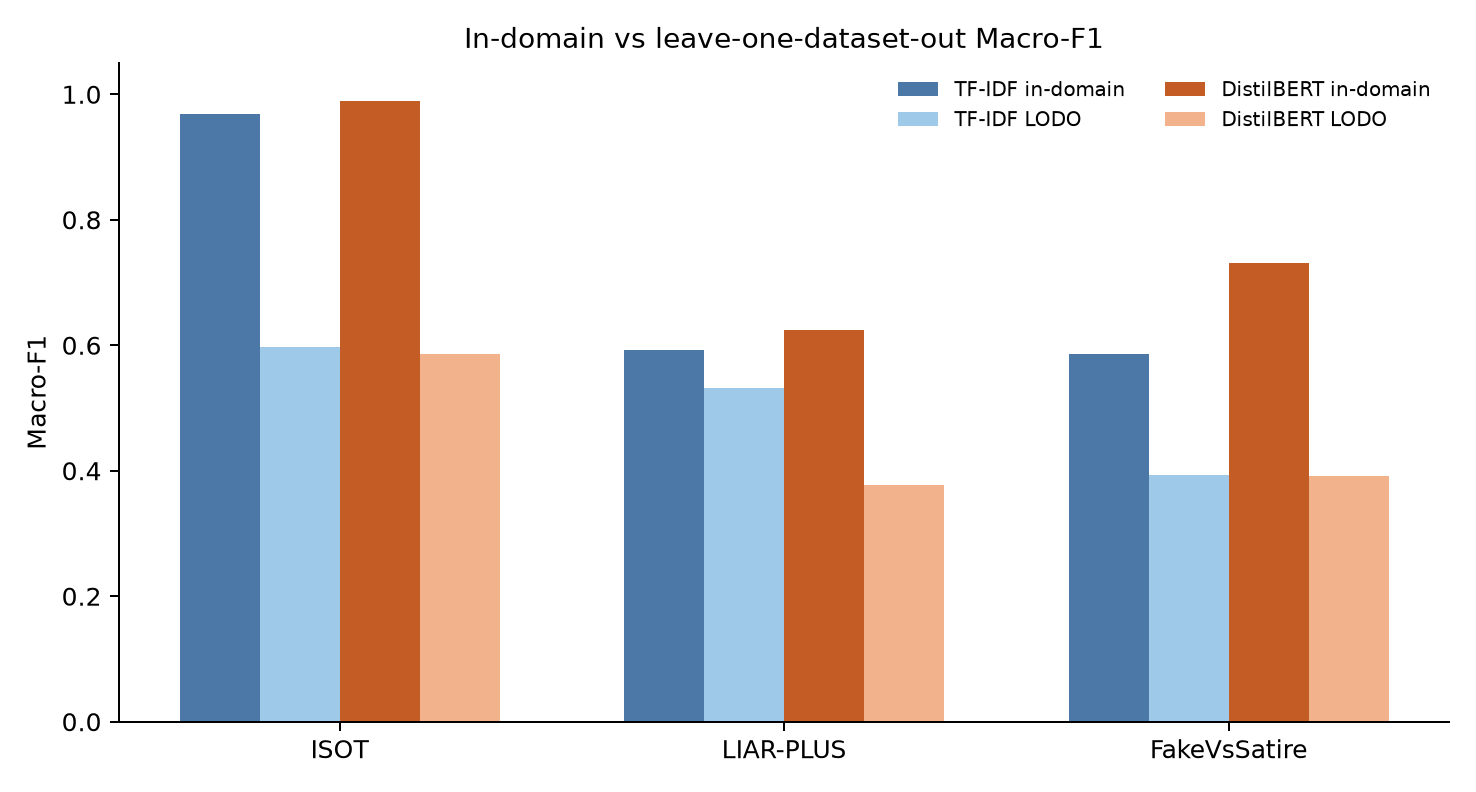
\includegraphics[width=\columnwidth]{../results/analysis/figures/fig1_lodo_drop.png}
\caption{In-domain and LODO macro-F1 for the two locked models. Values match Table~\ref{tab:main}.}
\label{fig:drop}
\end{figure}

The abstention results use DistilBERT runs R4, R5, and R6 only. TF-IDF is not scored by this rule. At threshold 0.3 on ISOT, the model answers 11 of 900 rows (coverage 0.0122) with risk 0.2727. At 0.4 it answers 4 rows (coverage 0.0044) with risk 0.7500. At 0.5 it answers 2 rows (coverage 0.0022) with risk 1.0000. The forced error rate on all 900 rows is 0.3811. Refusing almost every row is not a repaired detector.

On LIAR-PLUS the same thresholds answer 1215, 1194, and 1180 of 1267 rows. Coverage is 0.9590, 0.9424, and 0.9313. Risk is 0.5457, 0.5419, and 0.5407, against a forced risk of 0.5462. The model stays confident and stays wrong at nearly the same rate. On Fake versus Satire, thresholds 0.3 and 0.4 answer all 73 rows (coverage 1.0000, risk 0.5753). Threshold 0.5 answers 71 rows (coverage 0.9726, risk 0.5775). Figure~\ref{fig:abs} shows coverage beside risk.

\begin{figure}[t]
\centering
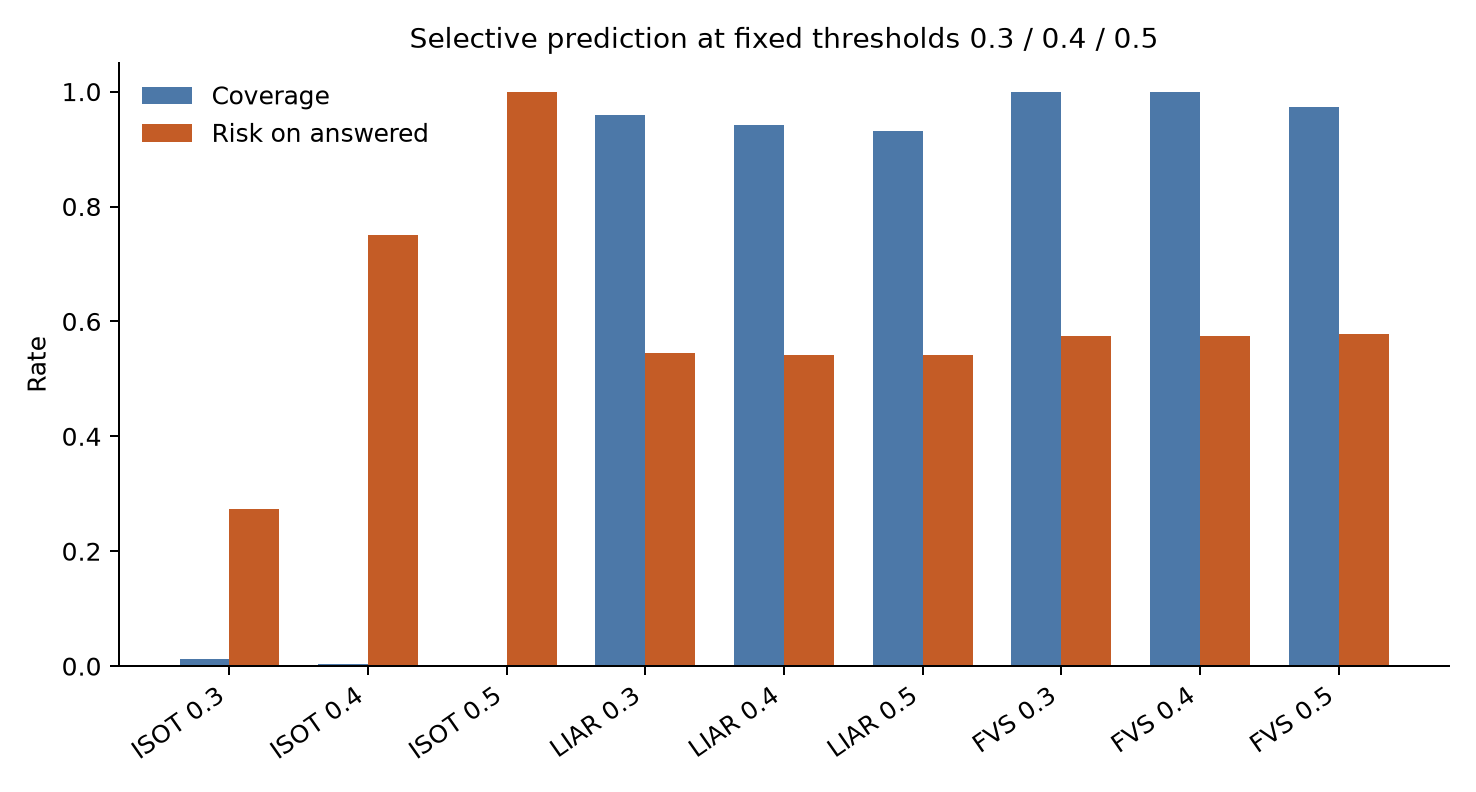
\includegraphics[width=\columnwidth]{../results/analysis/figures/fig2_abstention.png}
\caption{Coverage and risk for DistilBERT LODO predictions at thresholds 0.3, 0.4, and 0.5. The analysis script computed these quantities from saved probabilities.}
\label{fig:abs}
\end{figure}

LoRA does not close the gap. From R5, guided adaptation reaches macro-F1 0.3814 and accuracy 0.4546, a macro-F1 change of 0.0036 from 0.3778. Random adaptation reaches 0.3780 and accuracy 0.4530, a change of 0.0003. From R6, both guided and random adaptation stay at macro-F1 0.3917 and accuracy 0.4247, a change of 0.0000. Guided selection is skewed: 13 class-0 and 3 class-1 rows for LIAR-PLUS, and 2 class-0 and 14 class-1 rows for Fake versus Satire. Random selection is 8 and 8, and 9 and 7. Figure~\ref{fig:lora} shows the source bar and the adapted bar at nearly the same height.

\begin{figure}[t]
\centering
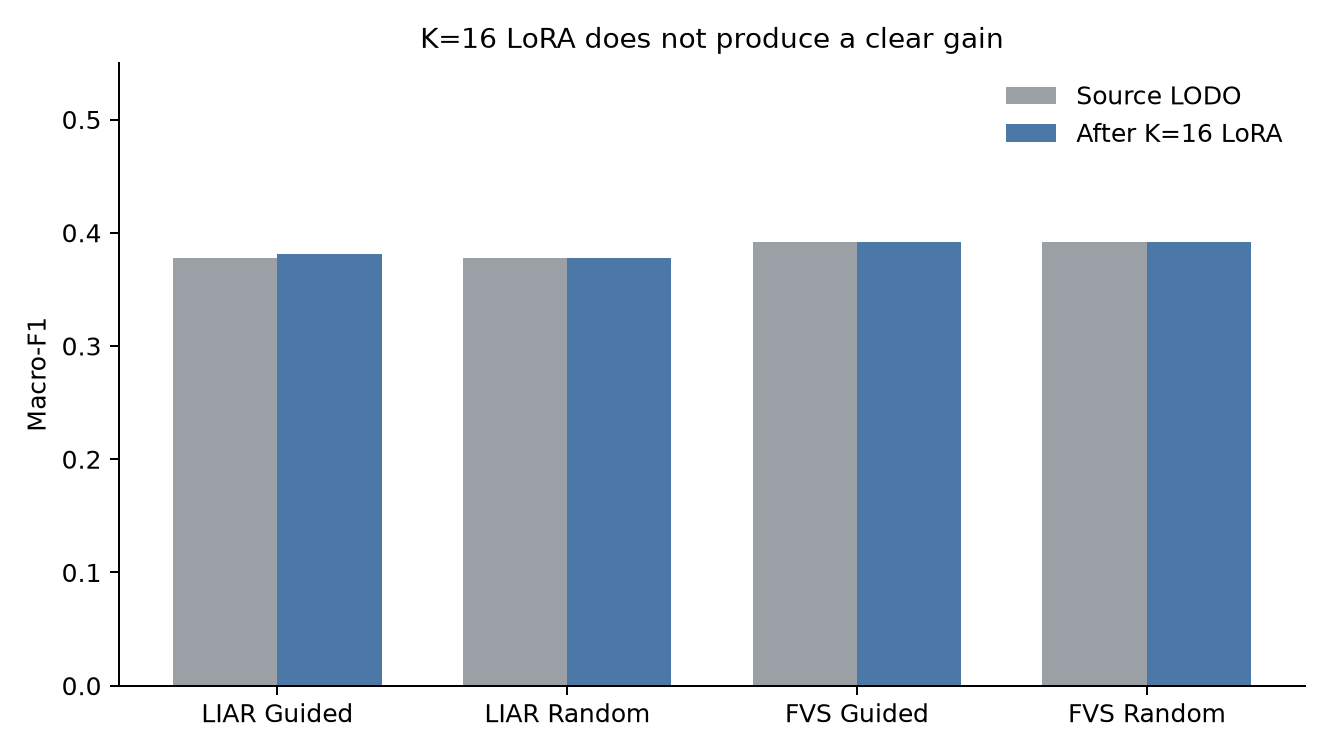
\includegraphics[width=\columnwidth]{../results/analysis/figures/fig3_lora.png}
\caption{Macro-F1 before and after K=16 LoRA. Source values are the R5 and R6 LODO scores. Adapted values are R7--R10.}
\label{fig:lora}
\end{figure}

The nine-source DistilBERT LODO macro-F1 on the original three tests is 0.6677 for ISOT (19,135 training rows), 0.3544 for LIAR-PLUS (13,127 training rows), and 0.7103 for Fake versus Satire (23,001 training rows). Relative to the two-source DistilBERT scores of 0.5867, 0.3778, and 0.3917, the extra sources coincide with a higher score on ISOT and Fake versus Satire and a lower score on LIAR-PLUS. These three numbers come from \texttt{train\_lodo10.py}. They do not replace Table~\ref{tab:main}.

\subsection{Systems results}
Table~\ref{tab:time} lists the training time stored for each locked neural job. The field is \texttt{train\_seconds\_this\_invocation}. For every run R1--R10 the saved \texttt{resumed\_from} value is null, so the number is the recorded training call, including that call's own checkpoint work, and not a separate measurement of tokens per second. No latency or throughput figure was saved, so none is reported. Fit times for the six locked TF-IDF runs are not present in the saved analysis tables, so they are omitted rather than reconstructed.

\begin{table}[t]
\caption{Recorded DistilBERT and LoRA training seconds for the locked jobs.}
\label{tab:time}
\centering
\scriptsize
\begin{tabular}{llrr}
\hline
Run & Job & Train rows & Seconds \\
\hline
R1 & DistilBERT, ISOT in-domain & 4200 & 125.1 \\
R2 & DistilBERT, LIAR-PLUS in-domain & 10208 & 309.1 \\
R3 & DistilBERT, satire in-domain & 334 & 9.7 \\
R4 & DistilBERT, LODO to ISOT & 10542 & 324.7 \\
R5 & DistilBERT, LODO to LIAR-PLUS & 4534 & 138.8 \\
R6 & DistilBERT, LODO to satire & 14408 & 567.1 \\
R7 & Guided LoRA from R5 & 16 & 0.5 \\
R8 & Guided LoRA from R6 & 16 & 0.3 \\
R9 & Random LoRA from R5 & 16 & 0.3 \\
R10 & Random LoRA from R6 & 16 & 0.3 \\
\hline
\end{tabular}
\end{table}

The smoke log records a different job: resume from step 10 to step 20 on 64 ISOT training rows, 1.9 seconds including load and save, and a peak allocation of 1.273 GiB. That job is a restart check. It is not one of the scored rows in Table~\ref{tab:main}.

The ten nine-source LODO training calls store their own \texttt{train\_seconds} values. The shortest is the LIAR-PLUS target at 344.2 seconds. The longest is the Horne target at 969.5 seconds. Those times belong to the extra script, not to R1--R10.

\section{Conclusion and Future Work}
On the saved test files, DistilBERT macro-F1 is 0.9889, 0.6238, and 0.7312 in-domain, and 0.5867, 0.3778, and 0.3917 under leave-one-dataset-out. TF-IDF with logistic regression is higher on all three leave-one-dataset-out targets in this run. Abstention at 0.3, 0.4, and 0.5 does not restore the DistilBERT LODO scores: ISOT is almost entirely refused, while LIAR-PLUS and Fake versus Satire are mostly answered at a risk close to the forced prediction. K=16 LoRA changes LIAR-PLUS macro-F1 from 0.3778 to 0.3814 (guided) and 0.3780 (random), and leaves Fake versus Satire at 0.3917. A separate nine-source DistilBERT run records 0.6677, 0.3544, and 0.7103 on the same three tests and does not overwrite the locked runs.

One limit of the test is that every scored comparison uses a single seed. The Fake-versus-Satire test contains 73 rows, so a change as small as 0.0003 is a description of this file, not a significance claim. A later measurement can repeat the same splits with more seeds. It should keep target test labels out of training, threshold choice, and adapter selection, and it should keep any new run in a new file so the numbers in Table~\ref{tab:main} remain recoverable.

\begin{thebibliography}{9}
\bibitem{delloglio2026}
P.~Dell'Oglio, A.~Bondielli, F.~Marcelloni, and L.~C.~Passaro, ``An experimental comparison of the most popular approaches to fake news detection,'' \emph{Information Sciences}, vol.~745, Art.~no.~123407, 2026, doi: 10.1016/j.ins.2026.123407.

\bibitem{sanh2019}
V.~Sanh, L.~Debut, J.~Chaumond, and T.~Wolf, ``DistilBERT, a distilled version of BERT: Smaller, faster, cheaper and lighter,'' arXiv:1910.01108, 2019.

\bibitem{hu2022}
E.~J.~Hu \emph{et al.}, ``LoRA: Low-rank adaptation of large language models,'' in \emph{Proc. Int. Conf. Learn. Represent.}, 2022.

\bibitem{pedregosa2011}
F.~Pedregosa \emph{et al.}, ``Scikit-learn: Machine learning in Python,'' \emph{J. Mach. Learn. Res.}, vol.~12, pp.~2825--2830, 2011.

\bibitem{wolf2020}
T.~Wolf \emph{et al.}, ``Transformers: State-of-the-art natural language processing,'' in \emph{Proc. Conf. Empirical Methods Natural Language Process.: Syst. Demonstrations}, 2020, pp.~38--45.

\bibitem{isotuvic}
ISOT Research Lab, ``ISOT fake news dataset,'' Univ. Victoria. [Online]. Available: \url{https://onlineacademiccommunity.uvic.ca/isot/datasets/}

\bibitem{phoenyx83}
Phoenyx83, ``ISOT fake news dataset, fine-tuned 2022 variant.'' [Online]. Available: \url{https://huggingface.co/datasets/Phoenyx83/ISOT-Fake-News-Dataset-FineTuned-2022}

\bibitem{liarplus}
LIAR-PLUS claim files, used from \url{https://github.com/Tariq60/LIAR-PLUS}. The local TSV files were hash-checked against that repository on 6 October 2026.
\end{thebibliography}

\end{document}
